\section{Experiments} \label{sec:srslam:experiments}
We confirm the simulation results in a preliminary experimental study by mounting a Raspberry Pi camera to the tip of a soft segment~\cite{katzschmann2019dynamic}. The robotic segment is guided to follow three trajectories similar to the ones tested in simulation (see Section~\ref{sub:srslam:trajectories}). % in 3D space by pneumatically actuating its segment with a pressure regulator. 
A motion capture setup is employed to gather an accurate ground-truth on the shape of the segment.

\begin{figure*}
     \centering
     \subfigure[Experimental setup]{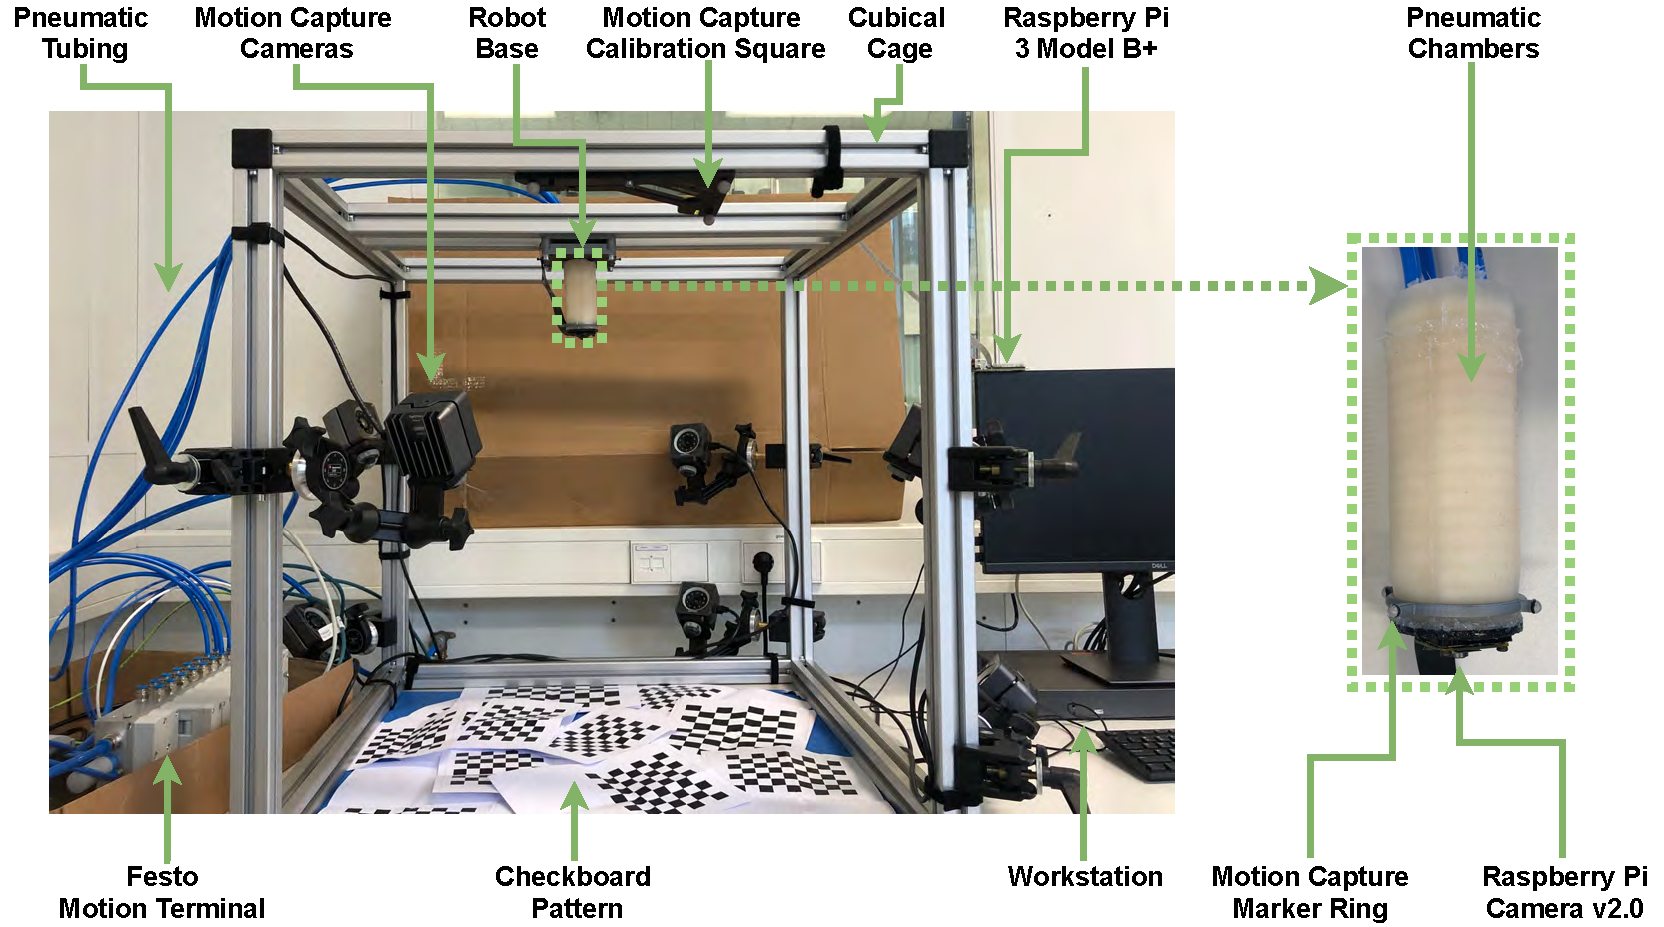
\includegraphics[height=.525\columnwidth]{srslam/figures/graphic_experimental_setup.drawio_v1_compressed.pdf} \label{fig:srslam:experimental_setup}}
     \subfigure[Trajectory 3]{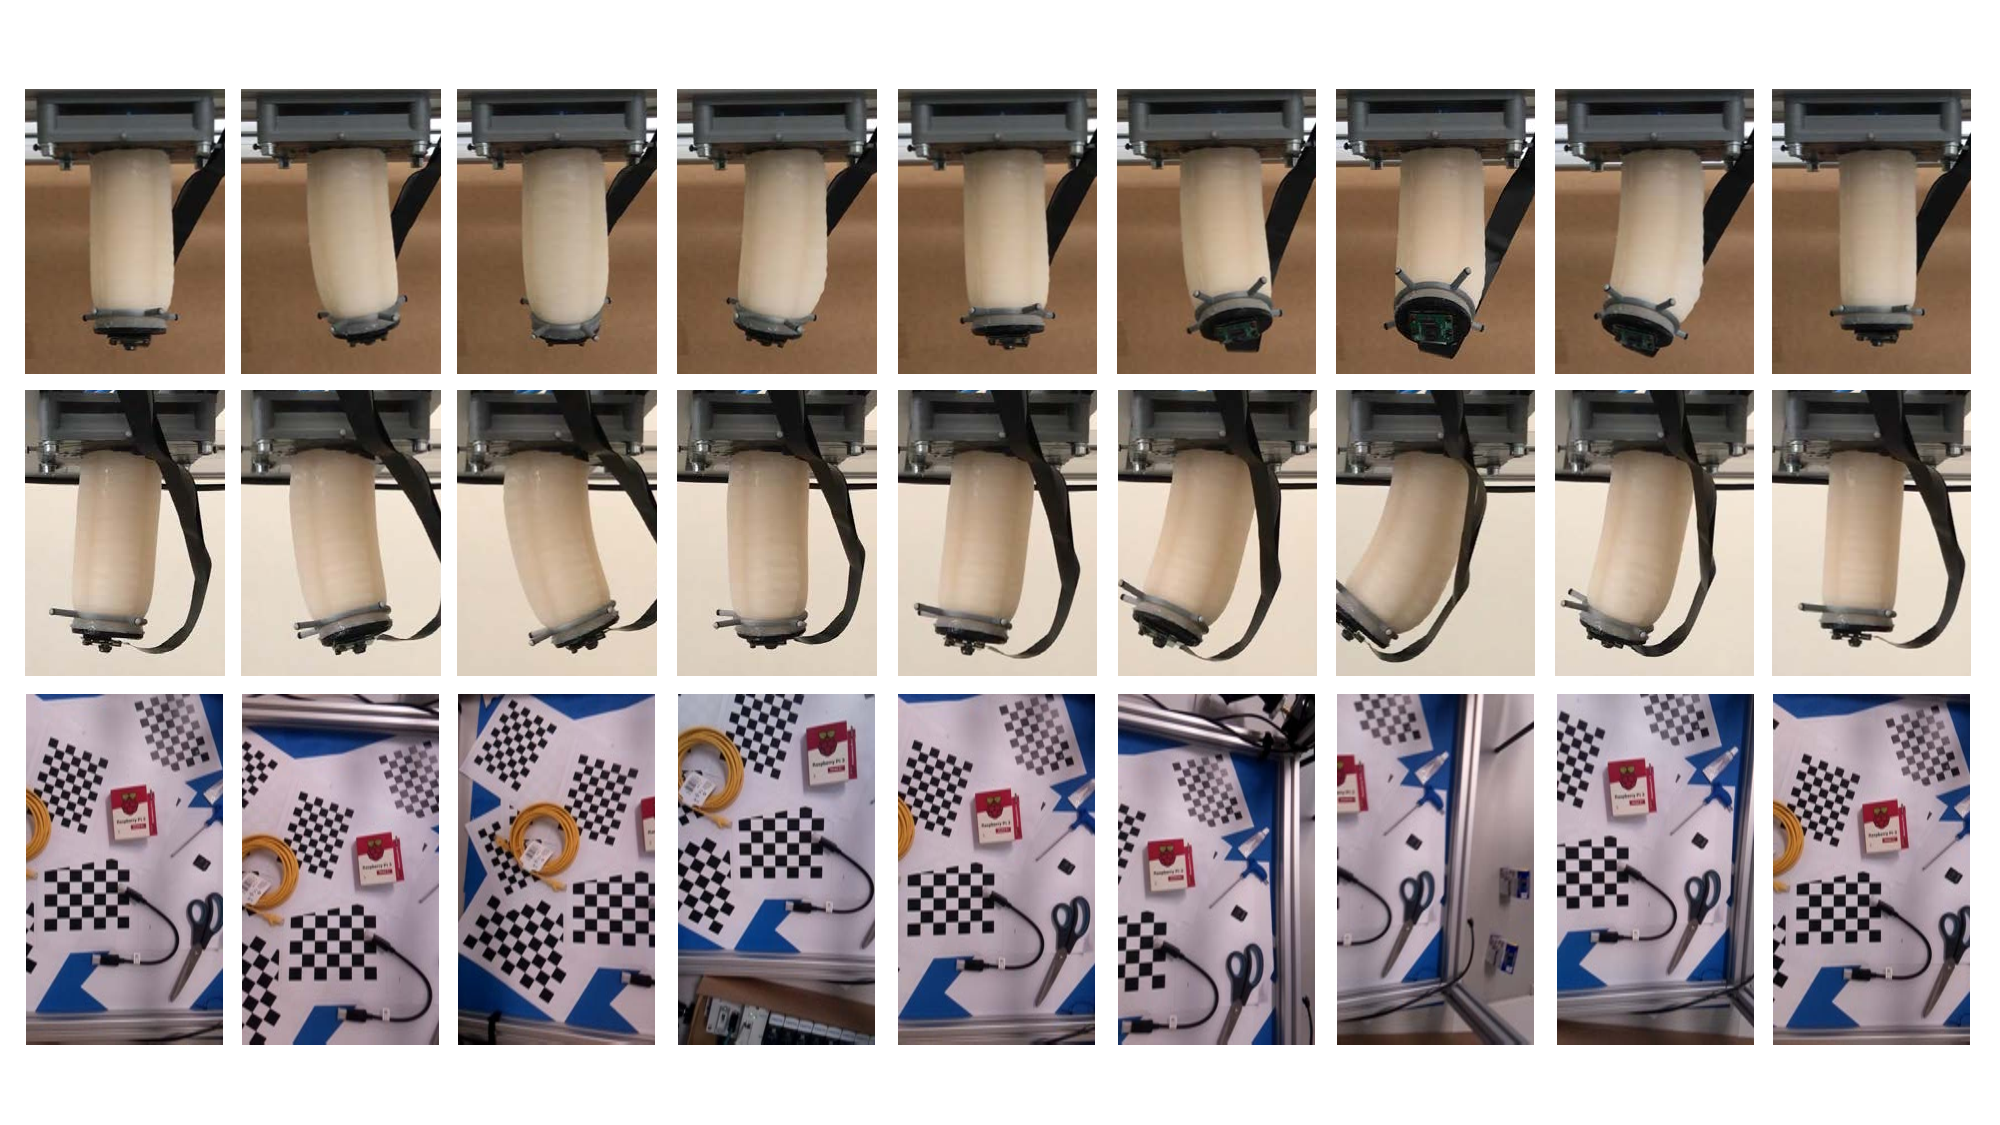
\includegraphics[height=.525\columnwidth]{srslam/figures/graphic_sequences_of_stills_lab_experiment_trajectory_3_compressed.pdf} \label{fig:srslam:graphic_sequences_of_stills_lab_experiment_trajectory_3}}
     \caption{ In Panel (a), a soft robotic segment is mounted to a cage with attached motion capture cameras. The segment is pneumatically actuated by a pressure regulator (Fest Motion Terminal). A Raspberry Pi camera v2.0 is attached to the tip of the segment and in a straight segment configuration looks down towards check-board patterns. Panel (b) depicts a sequence of stills showing the robot following trajectory 3 from two different vantage points. The second vantage point differs \SI{90}{\degree} from the first one. The third row displays a few representative frames as recorded by the camera attached to the tip of the segment.}
\end{figure*}

\subsection{Experimental setup}
% Segment and manufacturing
We show the experimental setup in Figure~\ref{fig:srslam:experimental_setup}.
We consider a soft robotic silicone segment consisting of four independently inflatable cavities. The segment has a cylindrical shape with a length $L_{0,1}$ of \SI{11}{cm} and a radius $d_1$ of \SI{21}{mm}. 
% We follow the fabrication procedure by Marchese et al.~\cite{marchese2015recipe} by casting Silicone into 3D-printed molds and block any silicon-flow into the air chambers with bees wax.
A 3D-printed ring with four motion capture markers is located near the tip of the segment.
%
% Camera and its attachment to the segment
We mount a Raspberry Pi camera module v2.0 to the tip of the segment.
This camera has a \SI{8}{MP} sensor and records frames at a sampling rate of \SI{30}{Hz} and a resolution of 1080p.
The focal length is \SI{3.04}{mm} and the field of view is $\SI{62.2}{\degree} \times \SI{48.8}{\degree}$.
The camera module is attached to a Raspberry Pi 3B+ single-board computer which saves the frames for later processing by the ORB-SLAM~\cite{mur2017orb} algorithm.
The camera is screwed onto a custom 3D-printed holder which in turn is glued with the tip plane of the segment.
%
% Actuation motion terminal, communication, commanding of pressures
The segment with its four air chambers is actuated with a proportional pressure regulator.
Tubing attached to the base of the segment connects each chamber with the assigned pneumatic valve of the pressure regulator.
%
% We apply a constant offset pressure $p_0$ to all chambers in straight configuration and subsequently synchronously increase the pressure $p_1$ in one chamber by $f_{\mathrm{p},x}$ and decrease the pressure in the opposite chamber $p_2$ by $f_{\mathrm{p},x}$ accordingly to cause a bending of the segment, in this case in x-direction.
% \begin{equation}
% \begin{split}
%     p_1 = p_0 - f_{\mathrm{p},x} \qquad p_2 = p_0 + f_{\mathrm{p},x}\\
%     p_3 = p_0 - f_{\mathrm{p},y} \qquad p_4 = p_0 + f_{\mathrm{p},y}
% \end{split}
% \end{equation}
% We map the desired configuration $\Delta_{x,1}$ and $\Delta_{y,1}$ given by the trajectories defined in \eqref{eq:srslam:trajectory_parametrization} in linear approximation to the commanded pressures
% \begin{equation}
%     f_{\mathrm{p},x} = a_x \; \Delta_{x,1} 
%     \qquad
%     f_{\mathrm{p},y} = a_y \; \Delta_{y,1}
%     \qquad
%     p_0 = a_{\delta L} \; \delta L_1
% \end{equation}
% where the proportional factors $a_{x}$, $a_{y}$ and $a_{\delta L}$ are experimentally determined and an elongation of the segment is reached through an increase in the offset pressure $p_0$.
% The pressure in each chamber is regulated by a Festo Motion Terminal using a factory-tuned PID controller.
% The commanded valve pressures are relayed via Modbus / TCP from our lab workstation to the Motion Terminal at a frequency of approximately \SI{10}{Hz}.
%
% Cage and environment
The segment is attached in up-side-down configuration to the top plane of a cubical cage of \SI{750}{mm} side length. For a straight segment, the camera is facing downwards towards the floor of the cage, which is covered by multiple printed checkerboard patterns.
%
% Motion capture system and cage
We acquire ground-truth pose information of the tip of the segment using an Optitrack motion capture system. %, consisting of eight PrimeX 13 cameras mounted to the previously mentioned cubic cage. 
The ground-truth poses of the tip of the segment are recorded at \SI{30}{Hz}. % analogous to the Raspberry Pi camera frames.
% Additionally, we also record the pose of the base of the segment allowing us to determine a ground-truth coordinate transformation $T_{0}^{1}$ from the base to the tip.
%
% Implementation of PCC projection and calibration sequence
%In contrast to the model we used in simulation, the real-world segment experiences an elongation caused by the application of pressure to the chambers. Accordingly, 
%
We also include the elongation of the segment $\delta L_1$ in the cost function \eqref{eq:srslam:cost_fun} of our optimization.
%
% Calibration sequence
To resemble the calibration sequence from simulation for the \gls{SLAM} map, we manually move the robot lateral into the x-coordinate direction before fixing it to the cage for the start of the experiments.

\subsection{Results}
Our experimental results reported in Table~\ref{tab:srslam:results_lab_experiments} and visualized for trajectory 3 in Figure~\ref{fig:srslam:experiments_t3_over_time} show translational relative \gls{RMSE} of between \SI{9}{\percent} and \SI{20}{\percent} for the three trajectories before optimization. 
The orientation of the z-axis of the tip is estimated with a mean error of approximately \SI{0.075}{\radian}.
The translational error is improved to between \SI{5}{\percent} and \SI{9}{\percent} after projection into the \gls{PCC}-kinematics. 
The optimization also slightly improves the rotational \gls{RMSE} by \SI{4}{\percent} to \SI{10}{\percent} relative to naive \gls{SLAM}.

The experimental results of the \gls{SLAM} algorithm are coherent with the simulations as the small segment length (\SI{11}{cm}) used in the experiments increases the translational errors as shown similarly in the simulations for a robot of length \SI{15}{cm}.
Even though the translational error is greatly reduced through optimization, it is still significantly higher than in simulation. Two reasons for this difference could be that a) the segment in simulation was modelled as in-extensible, while the real robot segment is extended via pneumatic pressurization, which introduces additional errors by \gls{SLAM} not accurately estimating the elongation movement and b) the real robot does not perfectly behave according to the \gls{CC} approximation as the simulated robot does.

% \begin{table}
% \centering
% \caption{ \textcolor{orange}{OLD RESULTS: }oReal-world results before and after optimization: the translational errors are stated through a relative \gls{RMSE} and the rotational errors with an absolute \gls{RMSE} taking into account the Frobenius norm of the rotation matrices.}
% \begin{tabular}{lclll}\toprule
% \textbf{Error category} & \textbf{Opt.} & \textbf{Traj. 1} & \textbf{Traj. 2} & \textbf{Traj. 3}\\
% \midrule
% Translation $e_\mathrm{t}$ Eq.~\eqref{eq:srslam:evaluation_translational_error} & No & $\SI{24.8}{\percent}$ & $\SI{21.4}{\percent}$ & $\SI{9.5}{\percent}$ \\
% Translation $e_\mathrm{t}$ Eq.~\eqref{eq:srslam:evaluation_translational_error} & Yes & $\SI{11.4}{\percent}$ & $\SI{13.0}{\percent}$ & $\SI{4.5}{\percent}$ \\
% \midrule
% Rotation $e_\mathrm{R}$ Eq.~\eqref{eq:srslam:evaluation_rotational_error} & No & $0.105$ & $0.131$ & $0.116$ \\
% Rotation $e_\mathrm{R}$ Eq.~\eqref{eq:srslam:evaluation_rotational_error} & Yes & $0.098$ & $0.125$ & $0.112$ \\
% \midrule
% \textcolor{orange}{Rotation $e_{\theta_z}$ Eq.~\eqref{eq:srslam:evaluation_angle_error}} & No & $0.105$ & $0.131$ & $0.116$ \\
% \textcolor{orange}{Rotation $e_{\theta_z}$ Eq.~\eqref{eq:srslam:evaluation_angle_error}} & Yes & $0.098$ & $0.125$ & $0.112$ \\
% \bottomrule
% \end{tabular}
% \label{tab:srslam:results_lab_experiments}
% \end{table}

\begin{table}
\centering
\caption{ Real-world results before and after optimization. The translational errors are stated through a relative \gls{RMSE} as described in \eqref{eq:srslam:evaluation_translational_error}. For rotation, we report both an absolute \gls{RMSE} computed with the Frobenius norm between the rotation matrices as stated in \eqref{eq:srslam:evaluation_rotational_error} and an angle error [rad] for the orientation of the z-axis of the tip of the segment as defined in \eqref{eq:srslam:evaluation_angle_error}. The results are averaged over two trials for each trajectory.}
\begin{tabular}{lclll}\toprule
\textbf{Error category} & \textbf{Opt.} & \textbf{Traj. 1} & \textbf{Traj. 2} & \textbf{Traj. 3}\\
\midrule
Translation $e_\mathrm{t}$ & No & $\SI{20.3}{\percent}$ & $\SI{14.2}{\percent}$ & $\SI{9.1}{\percent}$ \\
Translation $e_\mathrm{t}$ & Yes & $\SI{9.1}{\percent}$ & $\SI{8.9}{\percent}$ & $\SI{5.0}{\percent}$ \\
\midrule
Rotation $e_\mathrm{R}$ & No & $0.145$ & $0.103$ & $0.126$ \\
Rotation $e_\mathrm{R}$ & Yes & $0.130$ & $0.099$ & $0.120$ \\
\midrule
Rotation $e_{\theta_z}$ & No & $\SI{0.079}{\radian}$ & $\SI{0.068}{\radian}$ & $\SI{0.084}{\radian}$ \\
Rotation $e_{\theta_z}$ & Yes & $\SI{0.080}{\radian}$ & $\SI{0.067}{\radian}$ & $\SI{0.084}{\radian}$ \\
\bottomrule
\end{tabular}
\label{tab:srslam:results_lab_experiments}
\end{table}

\begin{figure}[ht]
    \centering
    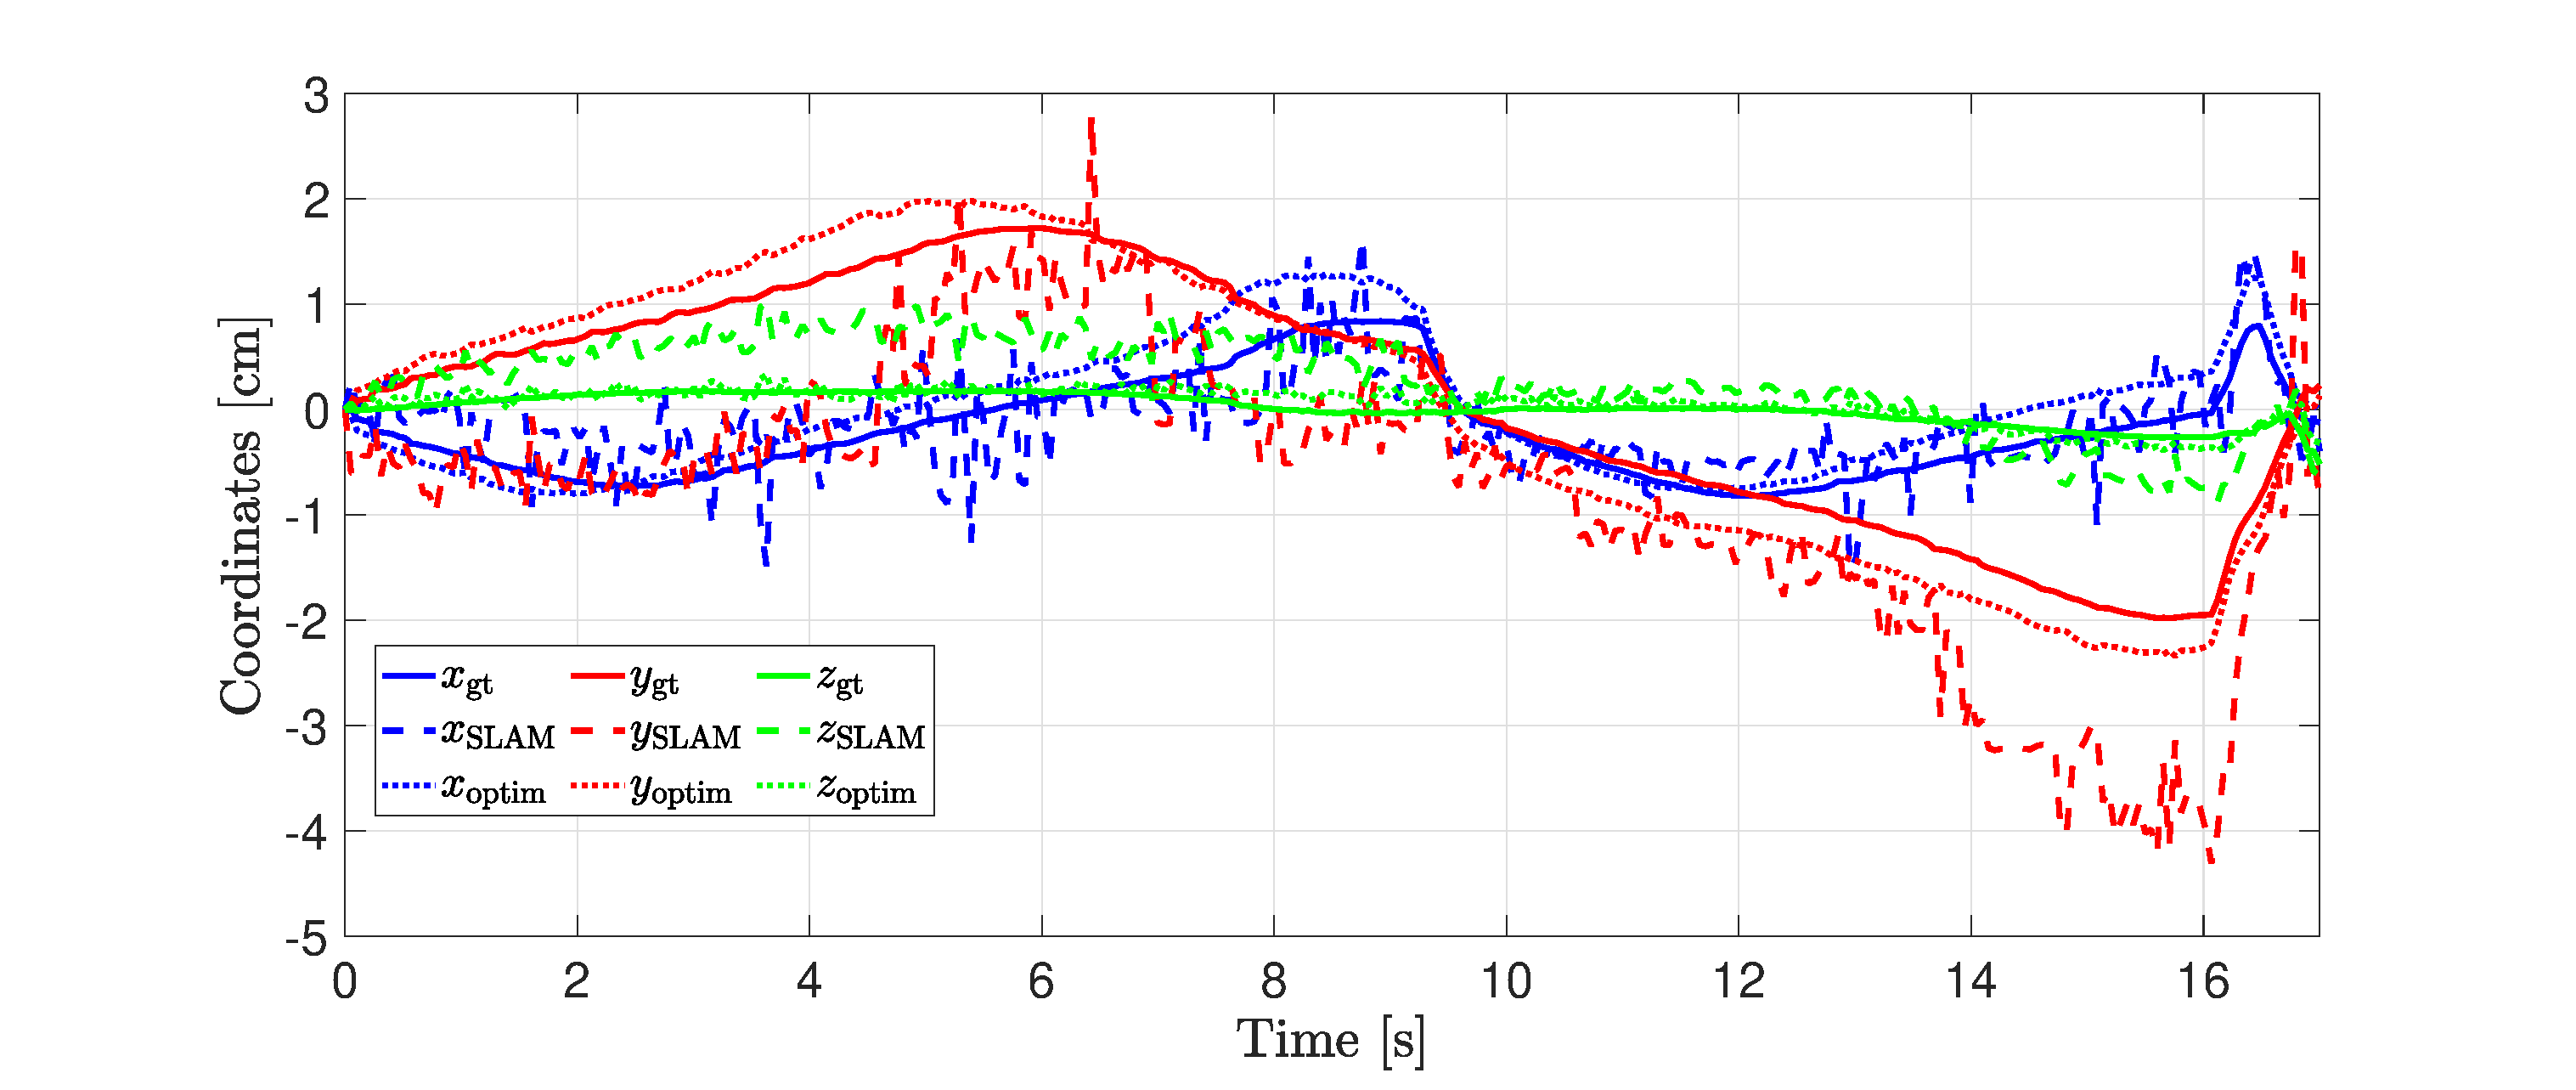
\includegraphics[width=0.9\columnwidth, trim={2cm 1.2cm 2cm 0}]{srslam/figures/vtem28_t3_coordinates.eps}\\
    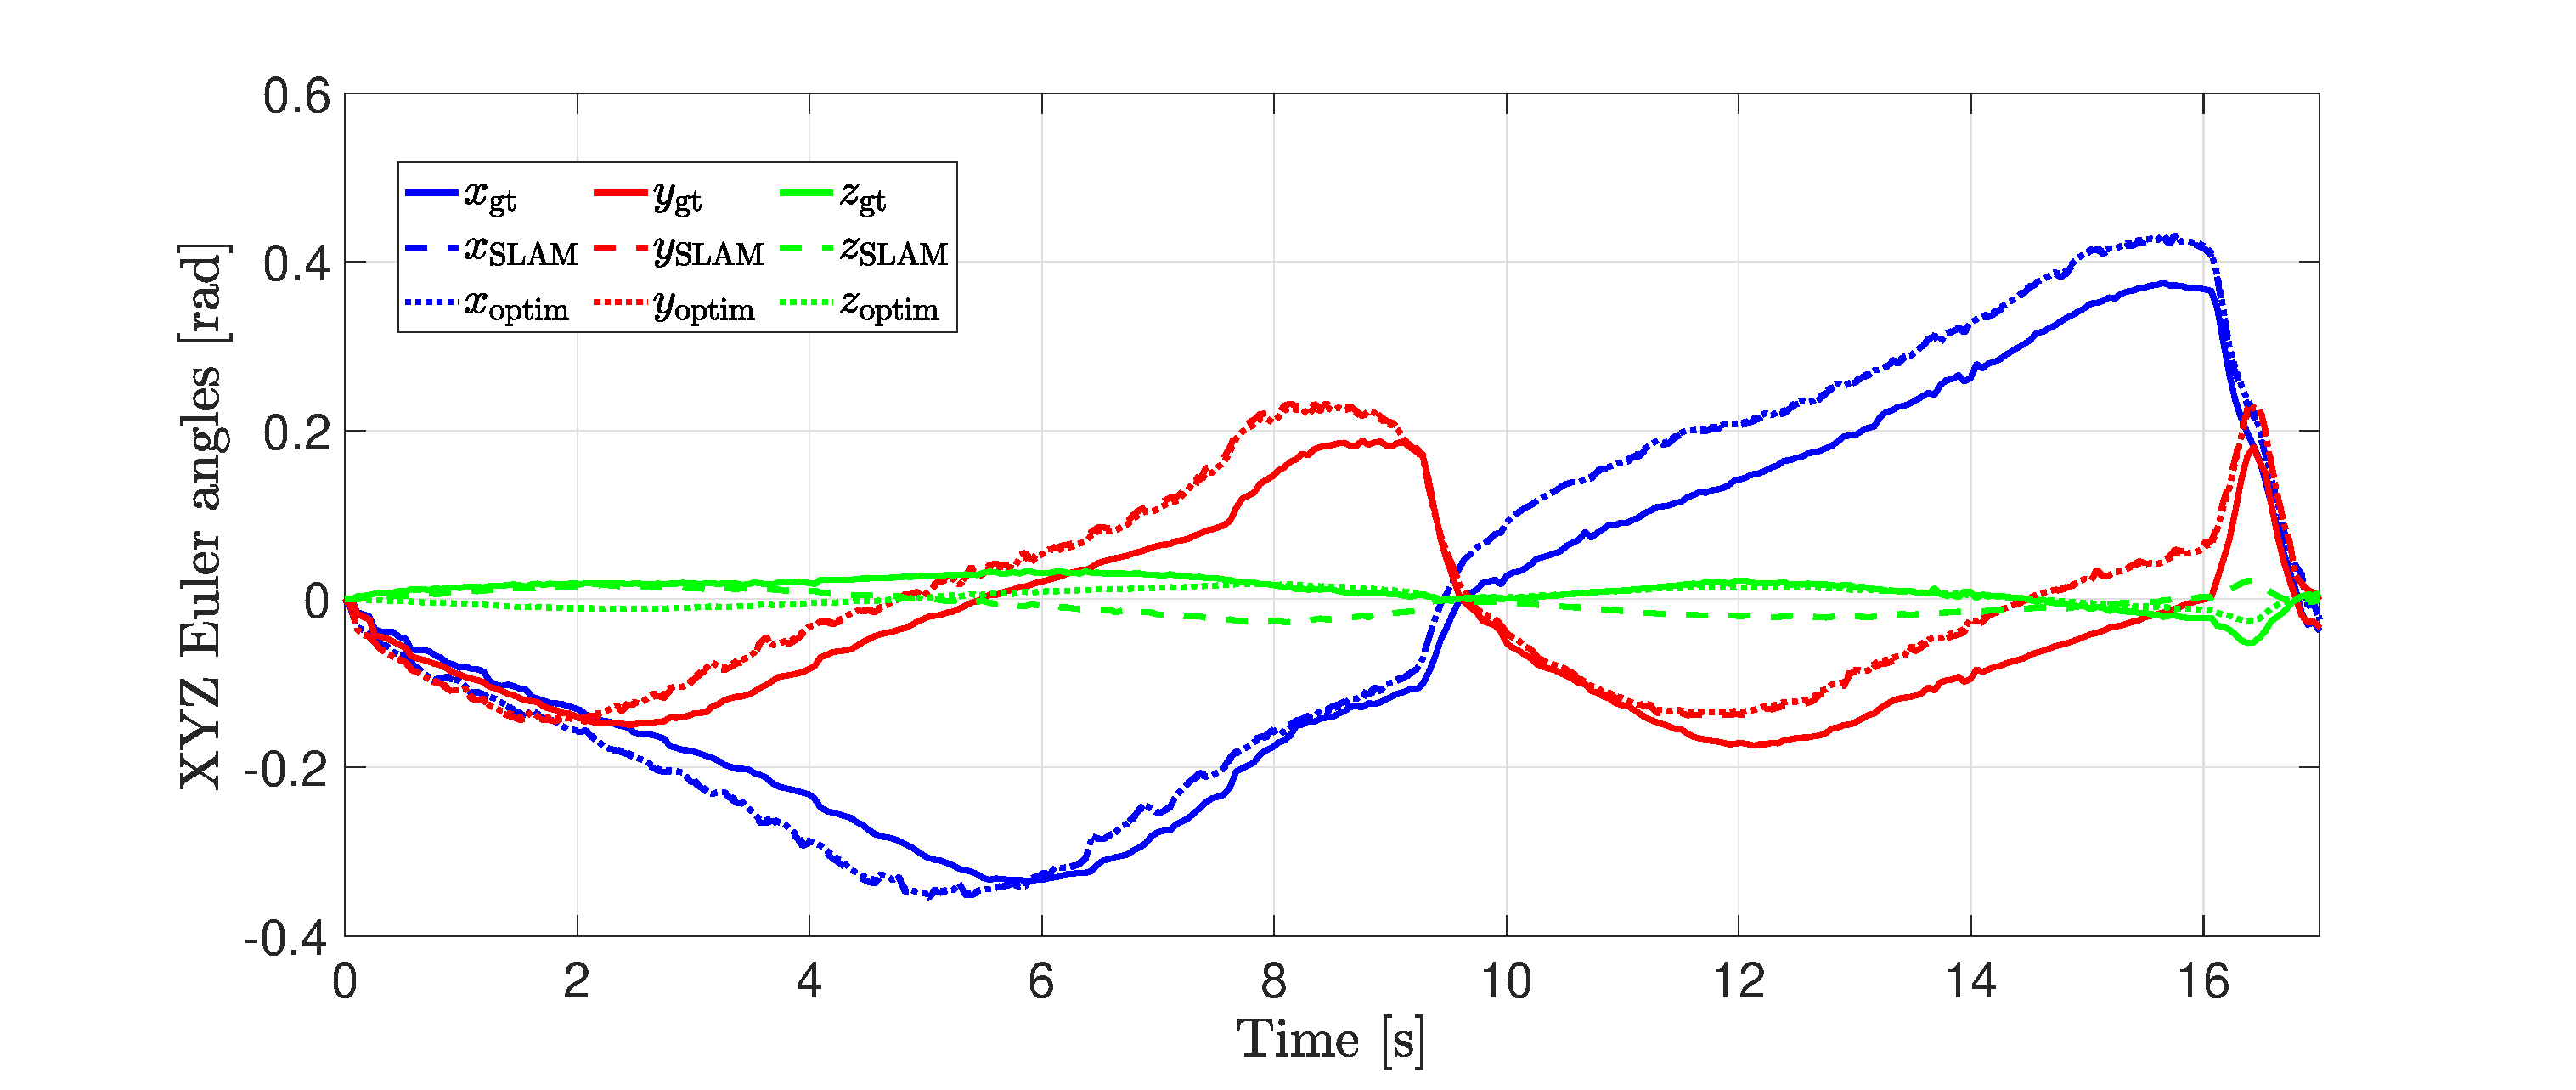
\includegraphics[width=0.9\columnwidth, trim={2cm 0 2cm 1.2cm}]{srslam/figures/vtem28_t3_angles.eps}
    \caption{ Experimental results for trajectory 3. Comparison between ground-truth (solid line), \gls{SLAM} (dashed line) and optimized through projection into \gls{PCC} kinematics (dotted line) for translation and orientation estimates.}
    \label{fig:srslam:experiments_t3_over_time}
\end{figure}

